\documentclass{standalone}
%% TikZ

\usepackage{tikz}

%% Libraries
\usetikzlibrary{positioning}
\usetikzlibrary{automata}
\usetikzlibrary{arrows}
\usetikzlibrary{matrix}
\usetikzlibrary{fit}
\usetikzlibrary{calc}
\usetikzlibrary{chains}
\usetikzlibrary{patterns}
\usetikzlibrary{shadows}
\usetikzlibrary{shapes.geometric}
\usetikzlibrary{shapes.symbols}
\usetikzlibrary{shapes.arrows}
\usetikzlibrary{shapes.callouts}
\usetikzlibrary{decorations.shapes}
\usetikzlibrary{decorations.pathreplacing}
\usetikzlibrary{decorations.pathmorphing}

% Related packages
\usepackage{pgfplots}
\usepackage{pgfplotstable}


\begin{document}
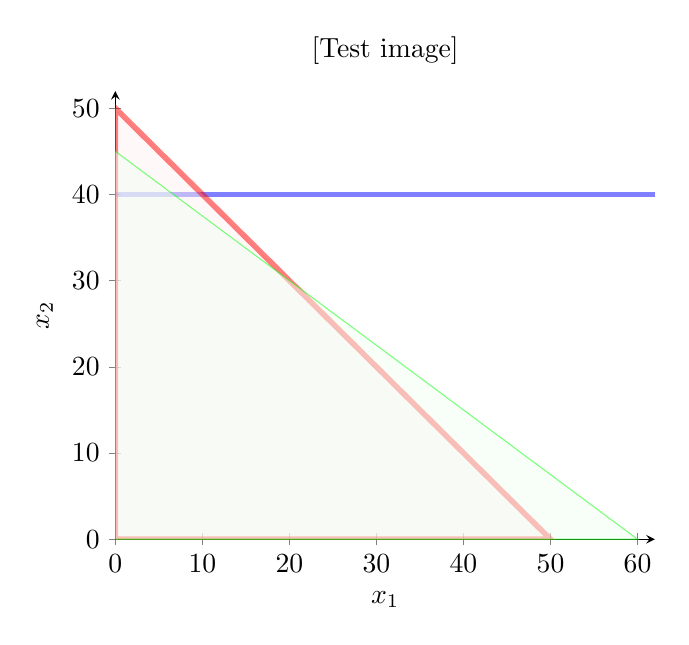
\begin{tikzpicture}
\begin{axis}[
	%height=5cm, width=6cm,
	title={[Test image]},
	xlabel=$x_1$,
	ylabel=$x_2$,
	xmax=62, ymax=52,
	axis x line=bottom,
	axis y line=left]
% constraints
\addplot[line width=2pt,color=blue,opacity=0.5] plot coordinates {
	(0, 40) (100, 40)
};
\addplot[line width=2pt,color=red,fill=red!5,opacity=0.5] plot coordinates {
	(0, 50) (50, 0)
} \closedcycle;
\addplot[color=green,fill=green!5,opacity=0.5] plot coordinates {
	(0, 45) (60, 0)
} \closedcycle;
\end{axis}
\end{tikzpicture}
\end{document}
